\section{Event selections}
\label{sec:event_selection}

The kinematic selection criteria used to define the signal region,
containing a sample of candidate signal events, as well as a number of
control regions in data, are described below. The criteria are based
on the physics objects defined by the event reconstruction algorithms
described in Section~\ref{sec:event_reconstruction}.

\subsection{Common preselection criteria}
\label{sec:preselection}

A number of beam and detector related effects, such as beam halo,
reconstruction failures, spurious detector noise, or event
misreconstruction due to detector inefficiencies, can lead to events
with anomolous levels of activity. These events, which can exhibit
large, non-physical values of \ETmiss, are rejected with high
efficiency by applying a range of dedicated
vetoes~\cite{1748-0221-5-03-T03014, CMS-NOTE-2010-012, cms-met}.

In order to suppress SM processes with genuine \ETmiss from neutrinos,
events containing an isolated electron or muon that satisfy $\Pt >
10\GeV$ and $\abs{\eta} < 2.5$ are vetoed. Events containing an
isolated photon with $\Pt > 25\GeV$ and $\abs{\eta} < 2.5$ are also
vetoed, in order to select only multijet final states. Furthermore,
events containing a single isolated track satisfying $\Pt > 10\GeV$
and $\abs{\eta} < 2.5$ are vetoed in order to reduce the background
contribution from final states containing hadronically-decaying tau
leptons.

Each jet $j_\text{i}$ is required to satisfy $\Pt^{j_\text{i}} >
40\GeV$ and $|\eta^{j_\text{i}}| < 3$. The highest \Pt jet in the
event is required to have $\Pt^{j_\text{1}} > 100\GeV$ and
$\abs{\eta^{j_\text{1}}} < 2.5$. The second highest \Pt jet in the
event is used to categorise events, as described in
Section~\ref{sec:categorisation}. If the jet satisfies
$\Pt^{j_\text{2}} > 100\GeV$, then this category of events is labelled
``symmetric'' and targets primarily topologies resulting from
pair-produced sparticles. If the jet satisfies $40 < \Pt^{j_\text{2}}
< 100\GeV$ or $\Pt^{j_\text{2}} < 40\GeV$, then these categories are
labelled as, respectively, ``asymmetric'' or ``monojet'' topologies,
which target models involving the direct production of stable, weakly
interacting, massive particles.

The mass scale of the physics processes being probed is characterised
by the scalar \Pt sum of the jets, defined as $\scalht =
\sum_{i=1}^{\njet} \Pt^{\,j_\text{i}}$, where \njet is the number of
jets within the experimental acceptance.  The magnitude of the
negative vector \ptvec sum of these jets, defined by $\HTmiss =
|-\sum_{i=1}^{\njet} \ptvec^{\,j_\text{i}}|$, is used to identify
events with a significant imbalance in transverse momentum. Events are
vetoed if any jet satisfies $\Pt > 40\GeV$ and $|\eta| > 3$ to ensure
that jets reconstructed in the forward regions of the detector do not
contribute significantly to \HTmiss.

An estimator of \ptvecmiss is given by the projection on the plane
perpendicular to the beams of the negative vector sum of the momenta
of all candidate particles in an event~\cite{cms-met}, as determined
by the PF algorithm. Its magnitude is referred to as \ETmiss. The
dimensionless variable $\HTmiss / \ETmiss$ is used to remove events
that contain several jets with transverse momenta below the jet \Pt
thresholds but an appreciable \Pt vector sum so as to contribute
significantly to \HTmiss relative to \ETmiss. This background is
typical of multijet events, which is suppressed by requiring $\HTmiss
/ \ETmiss < 1.25$. The requirement is imposed as part of the common
preselection criteria used to define all control samples, to minimise
potential systematic biases associated with the simulation modelling
for this variable. A high efficiency is maintained for SM or
new-physics processes that produce unobserved particles, which are
characterised by large values of \ptvecmiss and values of $\HTmiss /
\ETmiss$ close to unity.

Significant jet activity and missing transverse momentum in the event
is ensured by requiring $\scalht > 200\GeV$ and $\HTmiss > 130\GeV$,
respectively. These requirements complete the common preselection
criteria, summarised in Table~\ref{tab:selections}, used to define a
sample of all-jet events characterised by high activity and
appreciable missing transverse momentum.

\begin{table*}[tb]
  \topcaption{Summary of the event selection criteria and
    categorisation used to define the signal and control
    regions.}
  \label{tab:selections}
  \centering
  \footnotesize
  \begin{tabular}{ ll }
    \hline
    \multicolumn{2}{l}{\bf Common preselection}                                                                                                \\
    \ETmiss cleaning             & Filters related to beam and instrumental effects                                                                  \\ 
    Lepton/photon vetoes         & $\Pt > 10,\, 10,\, 25\GeV$ for isolated tracks, leptons, photons (respectively) and $\abs{\eta} < 2.5$            \\ 
    Jet $j_\text{i}$ acceptance  & Consider each jet $j_\text{i}$ that satisfies $\Pt^{j_\text{i}} > 40\GeV$ and $\abs{\eta^{j_\text{1}}} < 3$       \\
    Jet $j_\text{1}$ acceptance  & $\Pt^{j_\text{1}} > 100\GeV$ and $\abs{\eta^{j_\text{1}}} < 2.5$                                                  \\
    Jet $j_\text{2}$ acceptance  & 
    $\Pt^{j_\text{2}} < 40\GeV$ (monojet), 
    $40 < \Pt^{j_\text{2}} < 100\GeV$ (asymmetric), 
    $\Pt^{j_\text{2}} > 100\GeV$ (symmetric)                                                                                                         \\
    Forward jet veto             & Veto events containing jet satisfying $\Pt > 40\GeV$ and $\abs{\eta} > 3$                                         \\
    Jets below threshold         & $\HTmiss / \ETmiss < 1.25$                                                                                        \\
    Energy sums                  & $\scalht > 200\GeV$ and $\HTmiss > 130\GeV$                                                                       \\
    \hline
    \multicolumn{2}{l}{\bf Event categorisation}                                                                                                     \\
    \njet                        & 1 (monojet), 2, 3, 4, $\geq$5 (asymmetric), 2, 3, 4, $\geq$5 (symmetric)                                          \\
    \nb                          & 0, 1, 2, $\geq$3 ($\nb \leq \njet$)                                                                               \\
    \scalht (GeV)                & 200, 250, 300, 350, 400, 500, 600, $>$800\GeV (bins can be dropped/merged \vs \njet, Table~\ref{tab:binning}) \\
    \hline
    {\bf Signal region (SR)}     & Preselection +                                                                                                    \\
    QCD multijet rejection \quad & $\alphat > 0.65$, 0.60, 0.55, 0.53, 0.52, 0.52, 0.52 (mapped to \scalht bins in range $200 < \scalht < 800\GeV$)  \\
    QCD multijet rejection       & $\bdphi > 0.5$ (for the region $\scalht > 200\GeV$)                                                               \\[0.5ex]
    \hline
    {\bf Control regions (CR)}   & Preselection +                                                                                                    \\
    Multijet-enriched            & SR + $\HTmiss/\ETmiss > 1.25$ (inverted)                                                                          \\  
    \gj                          & 
    1$\gamma$ with $\Pt > 200\GeV$, $\abs{\eta} < 1.45$, 
    $\Delta R(\gamma,j_{\text{i}}) > 1.0$, 
    $\scalht > 400\GeV$, same \alphat req. as SR                                                                                                     \\[0.5ex]
    \mj                          & 
    1$\mu$ with $\Pt > 30\GeV$, $\abs{\eta} < 2.1$, 
    $I^{\mu}_\text{rel} < 0.1$, 
    $\Delta R(\mu,j_{\text{i}}) > 0.5$,
    $30 < m_\text{T}(\ptvec^\mu,\ptvecmiss) < 125\GeV$                                                                                               \\[0.5ex]
    \mmjpm                       & 
    2$\mu$ with $\Pt > 30\GeV$, $\abs{\eta} < 2.1$, 
    $I^{\mu}_\text{rel} < 0.1$, 
    $\Delta R(\mu_{1,2},j_{\text{i}}) > 0.5$, 
    $ \abs{m_{\mu\mu} - m_\text{Z}} < 25\GeV$                                                                                                        \\[0.5ex]
    \hline
  \end{tabular}
\end{table*}

\subsection{Event categorisation}
\label{sec:categorisation} 

Events selected by the common preselection criteria are categorised
according to \njet, the number of b-tagged jets \nb, and \scalht. Nine
categories in \njet are employed: the monojet topology ($\njet = 1$)
and four \njet bins (2, 3, 4, $\geq$5) for each of the asymmetric and
symmetric topologies. Events are also categorised by \nb (0, 1, 2,
$\geq$3), where \nb is bounded from above by \njet, resulting in 32
categories in terms of both \njet and \nb. For each (\njet,\nb)
category, events are binned according to \scalht: four 50\GeV bins at
low jet activity in the range $200 < \scalht < 400\GeV$, two 100\GeV
bins in the range $400 < \scalht < 600\GeV$, one bin covering the
region $600 < \scalht < 800\GeV$, and a final open bin for $\scalht >
800\GeV$. These categorisations are summarised in
Table~\ref{tab:selections}. The \scalht binning scheme is adapted
independently per (\njet,\nb) category by removing or merging bins to
satisfy a threshold on the minimum number of data events in the
control regions, which are used to estimate SM backgrounds, provide
checks, and validate assumptions within the methods. The lower bounds
of the first and final (open) bins in \scalht are summarised in
Table~\ref{tab:binning}. In summary, the search employs a
categorisation scheme for events that results in 191 bins, defined in
terms of \njet, \nb, and \scalht.

\newcommand{\dash}{\multicolumn{1}{c}{-}}
\begin{table}[tb]
  \topcaption{Summary of the lower bounds of the first and final bins
    in \scalht (the latter in parentheses) as a function of \njet and
    \nb.} 
  \label{tab:binning}
  \centering
  \footnotesize
  \begin{tabular}{ lrrrr }
    \hline
%    \njet                   & \multicolumn{4}{c}{\nb}                                           \\
%    \cline{2-5}
%                            & 0         & 1         & 2         & $\geq$3                       \\
    $\njet \backslash\, \nb$ & 0         & 1         & 2         & $\geq$3                       \\
    \hline
    \multicolumn{5}{l}{\bf Monojet}                                                              \\
    1                        & 200 (600) & 200 (500) & \dash     & \dash                         \\
    \multicolumn{5}{l}{\bf Asymmetric}                                                           \\
    2                        & 200 (600) & 200 (500) & 200 (400) & \dash                         \\
    3                        & 200 (600) & 200 (600) & 200 (500) & 200 (300)                     \\
    4                        & 200 (600) & 200 (600) & 200 (600) & 250 (400)                     \\
    $\geq$5                  & 250 (600) & 250 (600) & 250 (600) & 300 (500)                     \\
    \multicolumn{5}{l}{\bf Symmetric}                                                            \\
    2                        & 200 (800) & 200 (800) & 200 (600) & \dash                         \\
    3                        & 200 (800) & 250 (800) & 250 (800) & \phantom{0}-\phantom{0} (250) \\
    4                        & 300 (800) & 300 (800) & 300 (800) & 300 (800)                     \\
    $\geq$5                  & 350 (800) & 350 (800) & 350 (800) & 350 (800)                     \\
    \hline
  \end{tabular}
\end{table}

\subsection{Signal region}
\label{sec:signal_region} 

For events satisfying the common preselection criteria described
above, the multijet background dominates over all other SM
backgrounds. Several variables are employed to reduce the multijet
contribution to a negligible level with respect to other SM
backgrounds.

The dimensionless kinematic variable \alphat~\cite{Randall:2008rw,
  RA1Paper}, defined in Equ.~\ref{eq:alphat}, is used to provide
discrimination against multijet events that do not contain significant
\ptvecmiss or that contain large \ptvecmiss only because of transverse
momentum mismeasurements, while retaining sensitivity to new-physics
events with significant \ptvecmiss. The \alphat variable depends
solely on the transverse component of jet four-momenta
%the transverse energies and azimuthal angles of jets, 
and is intrinsically robust against the presence of jet energy
mismeasurements in multijet systems. For events containing only two
jets, \alphat is defined as $\alphat = \Et^{\text j_2}/M_\text{T}$,
where $\Et = E\sin\theta$, with $E$ the energy of the jet and $\theta$
its polar angle with respect to the beam axis, $\Et^{\text j_2}$ is
the transverse energy of the jet with smaller \Et, and $M_\text{T}$ is
the transverse mass of the dijet system, defined as:

\begin{equation}
  \label{eq:mt}
  M_\text{T} = \sqrt{ \left( \sum_{i=1}^2 \Et^{\mathrm{j}_i}
    \right)^2 - \left( \sum_{i=1}^2 p_x^{\mathrm{j}_i} \right)^2 - \left(
      \sum_{i=1}^2 p_y^{\mathrm{j}_i} \right)^2}\, ,
\end{equation}

where $\Et^{\mathrm{j}_i}$, $p_x^{\mathrm{j}_i}$, and
$p_y^{\mathrm{j}_i}$ are, respectively, the transverse energy and $x$
or $y$ components of the transverse momentum of jet $\mathrm{j}_i$.

For a perfectly measured dijet event with $\Et^{\mathrm{j}_1} =
\Et^{\mathrm{j}_2}$ and the jets in the back-to-back configuration
($\Delta\phi = \pi$), and in the limit in which the momentum of each
jet is large compared with its mass, the value of \alphat is 0.5. For
an imbalance in the \Et of back-to-back jets, \alphat is reduced to a
value $<0.5$, which gives the variable its intrinsic
robustness. Values significantly greater than 0.5 are observed when
the two jets are not back-to-back and recoil against \ptvecmiss from
weakly interacting particles that escape the detector.

The definition of the \alphat variable can be generalised for events
with more than two jets~\cite{RA1Paper}. The mass scale for any
process is characterised through the scalar sum of the jet transverse
energies, defined as $\scalst = \sum_{i=1}^{N_\text{jet}}
|\vec{\Et}^{\mathrm{j}_i}|$, where $N_\text{jet}$ is the number of
jets with \Et above a predefined threshold.\footnote{The definition of
  \scalst should be contrasted with that of \scalht, the scalar sum of
  the jet tranverse {\it momenta}. }
% The estimator for \ptvecmiss is \HTmiss. 
For events with three or more jets, a pseudo-dijet system is formed by
combining the jets in the event into two pseudo-jets. The \scalst for
each of the two pseudo-jets is given by the scalar \Et sum of its
contributing jets. The combination chosen is the one that minimises
\dst, defined as the difference between these sums for the two
pseudo-jets.  This clustering criterion assumes a balanced-event
hypothesis, which provides strong separation between SM multijet
events and events with genuine \ptvecmiss. The \alphat definition can
be generalised to:

\begin{equation}
  \label{eq:alphat}
  \alphat = \frac{1}{2} \frac{\scalst -
    \dst}{\sqrt{(\scalst)^2 - (\HTmiss)^2}}.
\end{equation}

When jet energies are mismeasured, or there are neutrinos from
heavy-flavour quark decays, the magnitude of \HTmiss and \dst are
highly correlated. This correlation is much weaker for
R-parity-conserving SUSY events, where each of the two decay chains
produces an undetected LSP.

Multijet events populate the region $\alphat< 0.5$ and the $\alphat$
distribution is characterised by a sharp edge at 0.5, beyond which the
multijet event yield falls by several orders of magnitude. Multijet
events with extremely rare but large stochastic fluctuations in the
calorimetric measurements of jet energies can lead to values of
\alphat slightly above 0.5. The edge at 0.5 sharpens with increasing
\scalht for multijet events, primarily due to a corresponding increase
in the average jet energy and a consequent improvement in jet energy
resolution. 

For events containing at least two jets, thresholds on the minimum
allowed \alphat values are applied independent of \njet and \nb but
dependent on \scalht, for events that satisfy $200 < \scalht <
800\GeV$. The \alphat thresholds vary between 0.65 to 0.52 for,
respectively, the regions $200 < \scalht < 250\GeV$ and $400 < \scalht
< 800\GeV$. No requirement on \alphat is made for the region $\scalht
> 800\GeV$. The thresholds employed are summarised in
Table~\ref{tab:selections}. The \alphat thresholds are motivated both
by the trigger conditions used to record the candidate signal events,
described below, and by simulation-based studies and data-derived
estimates of the multijet background. 
%As a rule of thumb, an \alphat threshold can be converted to an
%``effective'' lower bound threshold on \HTmiss by forcing $\dst =
%0\GeV$. Hence, the \alphat thresholds convert to approximate minimum
%values of $110 < \HTmiss < 160\GeV$ for the range $200 < \scalht <
%800\GeV$.

An additional variable is based on the minimum azimuthal separation
between a jet and the negative vector \ptvec sum derived from all
other jets in the event~\cite{RA1Paper},

%\begin{equation}
%  \bdphi = \min_{\,\forall\, j_\text{k} \,\in\, \njet}
%  \Delta\phi(\ptvec^{\,j_\text{k}}, -\sum_{j_\text{i}\, =\, 1}^{\njet}
%  \ptvec^{\,j_\text{i}} + \ptvec^{\,j_\text{k}}).   
%  \label{eq:bdphi}
%\end{equation}

\begin{equation}
  \bdphi = \min_{\,\forall\, j_\text{k} \,\in\, \njet}
  \Delta\phi( -\ptvec^{\,j_\text{k}}, 
  \sum_{\substack{j_\text{i}\, =\, 1 \\ j_\text{i} \ne j_\text{k}}}^{\njet}
  \ptvec^{\,j_\text{i}}).   
  \label{eq:bdphi}
\end{equation}

This variable discriminates between final states with genuine
\ptvecmiss, \eg from the leptonic decay of the W boson, and energetic
multijet events that have significant \ptvecmiss through jet energy
mismeasurements or through the production of neutrinos, collinear with
the axis of a jet, from semileptonic heavy-flavour decays. Multijet
events populate the region $\bdphi < 0.5$, with the multijet
distribution peaking at a value of zero and falling approximately
exponentially over five orders of magnitude to the event level at a
value of $\bdphi \approx 0.5$, which is close to the radius parameter
value of 0.4 used by the anti-$k_\text{t}$ jet clustering
algorithm. Events with a genuine source of \ptvecmiss exhibit a long
tail in \bdphi with values as large as $\pi$. The \bdphi variable
provides comparable or improved performance in terms of discrimination
according to a simple signal-to-background metric for a wide range of
signal models with respect to more widely used variables such as:

\begin{equation}
  \Delta\phi_\text{min} = \min_{\,\forall\, j_\text{k} \,\in\, \njet}
  \Delta\phi(\ptvec^{\,j_\text{k}}, -\sum_{j_\text{i}\, =\, 1}^{\njet}
  \ptvec^{\,j_\text{i}}).
  \label{eq:dphi}
\end{equation}

%and $\min_{\,\forall\, j_\text{k} \,\in\, \njet}
%\Delta\phi(\ptvec^{j_\text{k}}, \ptvecmiss)$.

A requirement of $\bdphi > 0.5$ is sufficient to effectively suppress
the multijet background to a negligible level while maintaining high
efficency to new-physics signatures. The combined rejection power of
the \alphat and \bdphi requirements for the region $200 < \scalht <
800\GeV$ are sufficient to suppress multijet events to the few percent
level with respect to all other SM backgrounds in all \scalht bins for
all event categories of the signal region. For the region $\scalht >
800\GeV$, a similar control of the multijet background is achieved
solely with the $\bdphi > 0.5$ requirement.

\begin{figure*}[!h]
  \begin{center}
    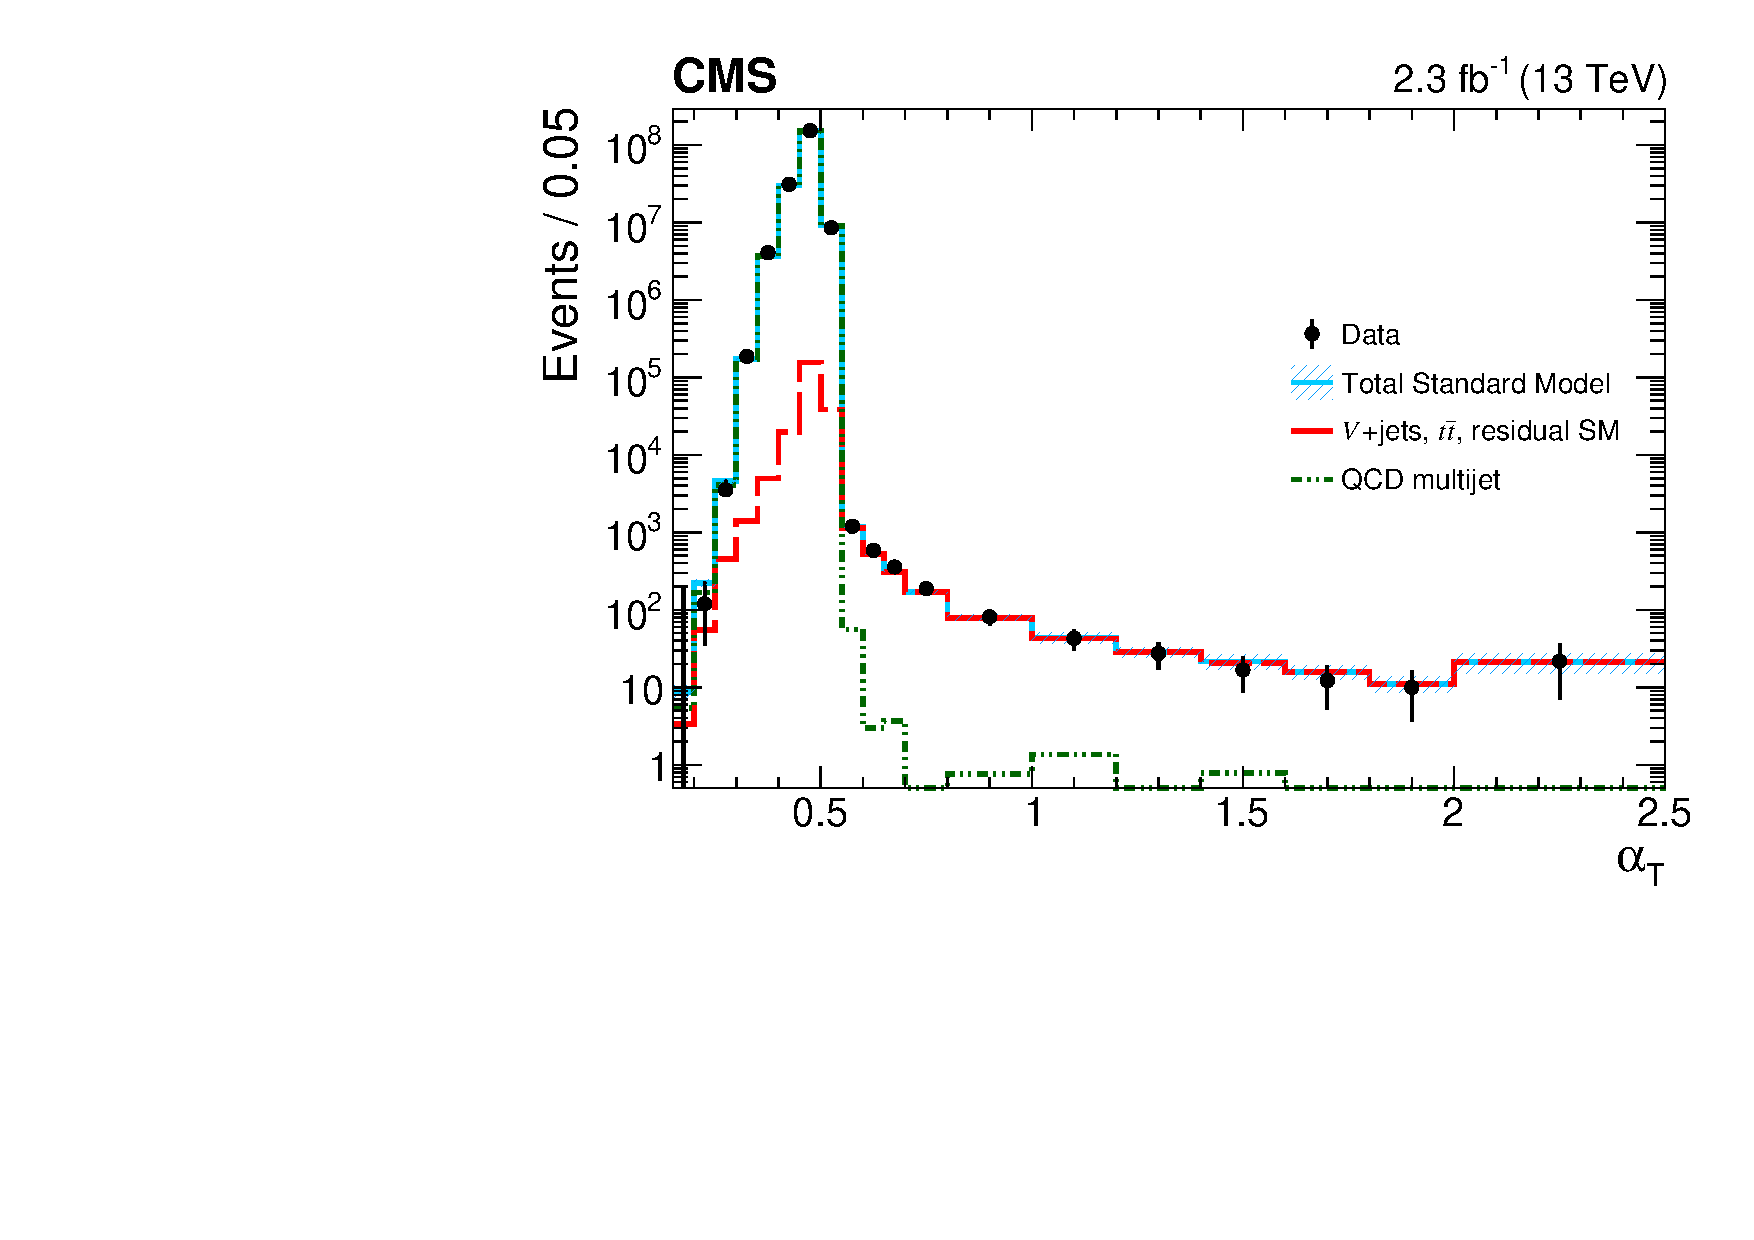
\includegraphics[width=0.49\textwidth]{figures/kine/v1/AlphaT_Paper} \,
    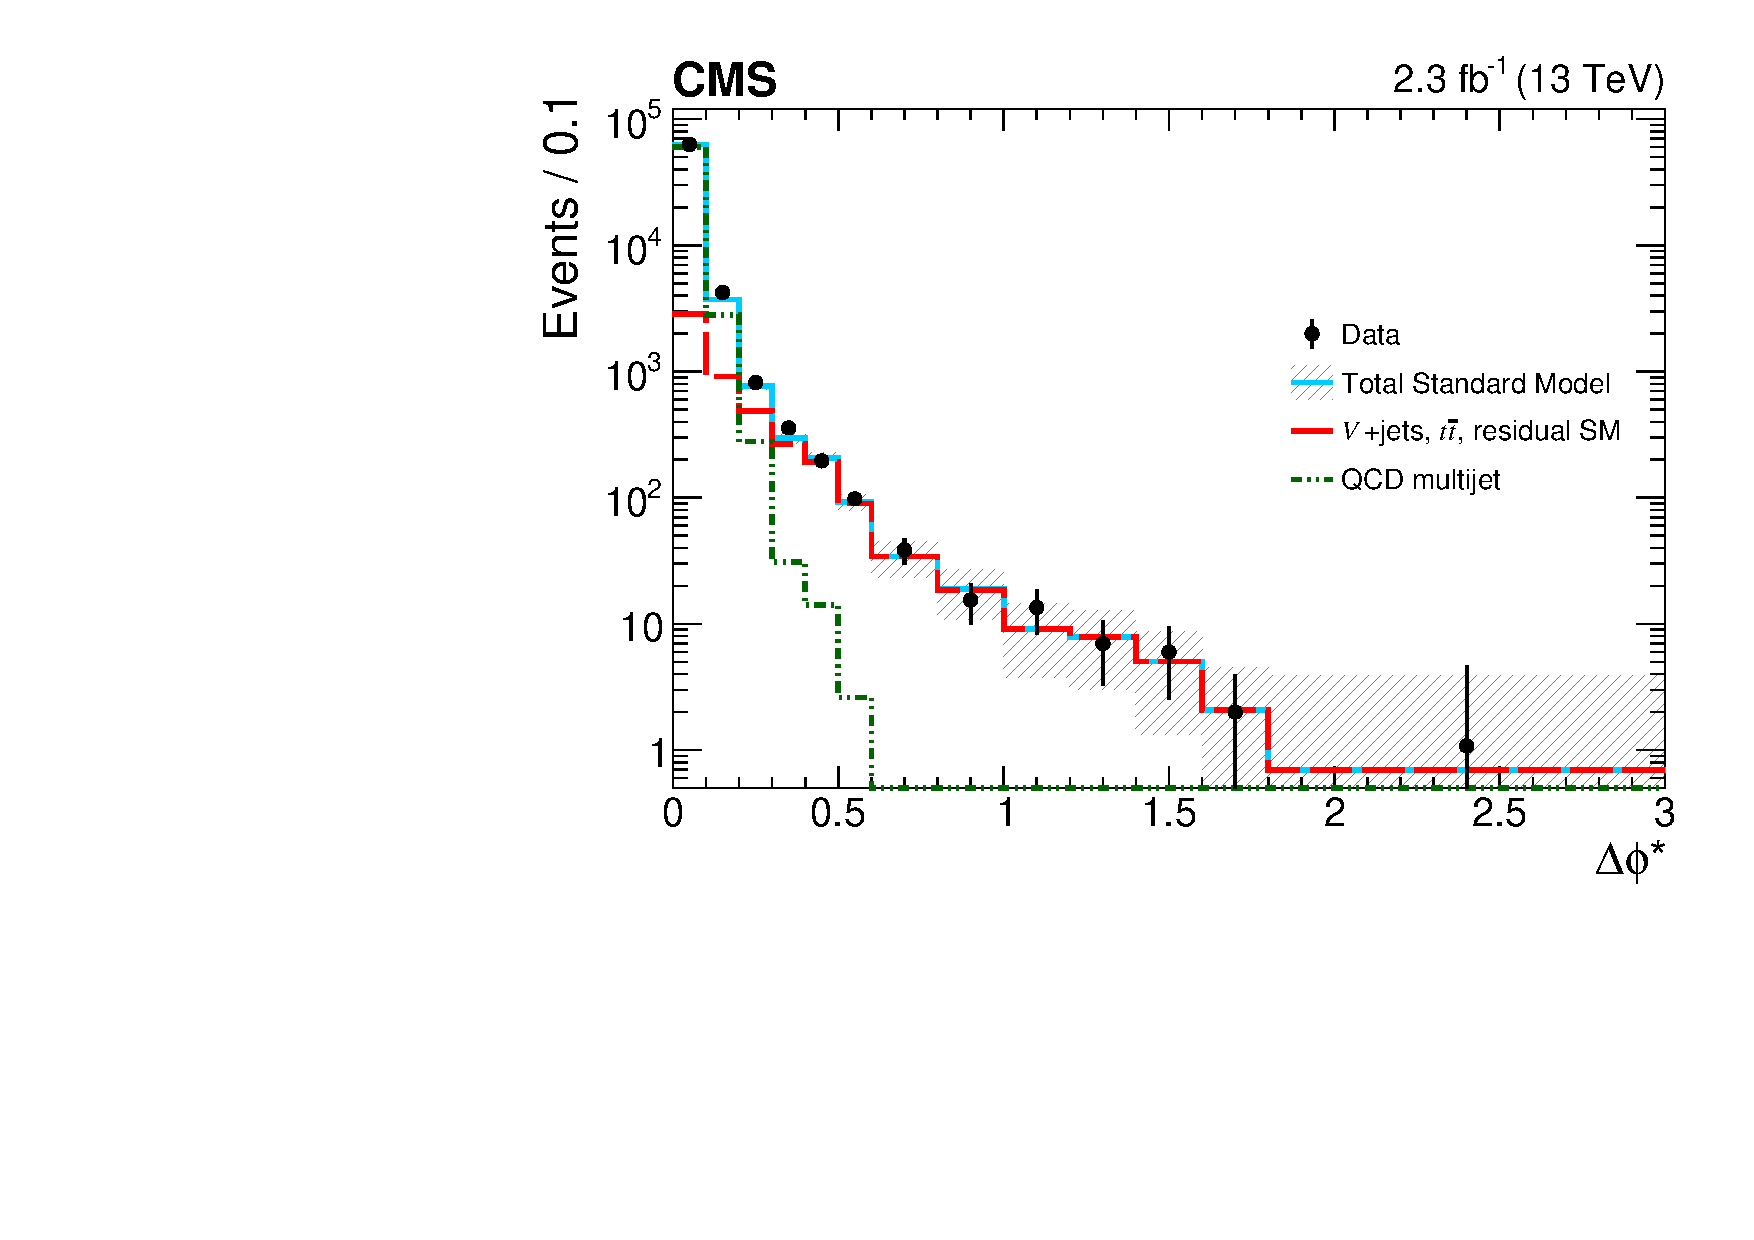
\includegraphics[width=0.49\textwidth]{figures/kine/v1/BDPhi_paper} \\
  \end{center}
  \caption{ (Left) The \alphat distribution observed in data for
    events that are recorded with an inclusive set of trigger
    conditions and satisfy either the common preselection criteria and
    $\alphat < 0.55$, or the full signal region selection criteria and
    $\alphat > 0.55$, as well as the additional requirement $\scalht >
    300\GeV$.  (Right) The \bdphi distribution observed in data for
    events that are recorded with an inclusive set of trigger
    conditions and satisfy the full signal region selection criteria
    for the region $\scalht > 800\GeV$.  The distributions for the QCD
    multijet backgrounds are determined from simulation while all
    other SM backgrounds (vector boson production in association with
    jets, \ttbar, and other residual contributions from rare SM
    processes) are estimated using a \mj data control sample.  These
    distributions illustrate the performance of these two variables in
    a kinematic phase space that is representative of the signal
    region. The statistical uncertainties for the multijet and SM
    expectations are represented by the hatched areas (visible only
    for statistically limited bins). The final bin of each
    distribution contains the overflow events.  }
  \label{fig:alphat-bdphi} 
\end{figure*}

Figure~\ref{fig:alphat-bdphi} illustrates the performance of the
\alphat and \bdphi variables, by showing their distributions observed
in data for events that satisfy all other signal region selection
criteria, as defined in Table~\ref{tab:selections}, and additional
requirements on \scalht. In the case of the \alphat distribution, the
events that satisfy $\alphat < 0.55$ must only fulfil the common
preselection criteria defined in Table~\ref{tab:selections}, no
\HTmiss requirement is made, and the events are recorded with an
inclusive set of trigger \scalht conditions that are independent of
the \alphat variable. In the case of the \bdphi distribution, events
are also recorded with an inclusive set of trigger conditions, and
must satisfy the full signal region selection criteria for the region
$\scalht > 800\GeV$. The contribution from multijet events is observed
to fall by five orders of magnitude for both variables.

The aforementioned requirements complete the event selection criteria
for the signal region. The \alphat and \bdphi requirements, in
conjunction with the common preselection requirements $\HTmiss >
130\GeV$ and $\HTmiss / \ETmiss < 1.25$, provide strong rejection
power against contributions from multijet events. Finally, a
modification to the \bdphi variable, which considers soft jets with
$\Pt > 25\GeV$ and is henceforth labeled $\bdphimod$, is used as a
control variable in data to identify multijet contributions arising
from instrumental effects, such as inefficient detector elements or
detector noise. The axis of any jet that satisfies $\bdphimod < 0.5$
is used to identify localised behaviour in the ($\eta$,$\phi$) plane,
which may be indicative of instrumental defects. No significant
anomolies are observed in the sample of candidate signal events
following the application of the dedicated vetoes mentioned in
Section~\ref{sec:preselection}.

%Signal candidate events are recorded with multiple jet-based trigger
%conditions that utilise calculations of \scalht and \alphat, and
%events are required to satisfy predetermined thresholds for both
%variables, as well as a threshold on the mean \Pt of the two highest
%\Pt jets.

Multiple trigger conditions are employed in combination to record
signal candidate events. A set of trigger conditions utilise
calculations of both \scalht and \alphat to record events with two or
more jets. An event is recorded if it satisfies any of the following
pairs of (\scalht,\alphat) thresholds, (200,0.57), (250,0.55),
(300,0.53), (350,0.52), or (400,0.51), as well as a requirement on the
mean value of the two highest \Pt jets, $\langle\Pt^{j_\text{1}} +
\Pt^{j_\text{2}}\rangle > 90\GeV$. These requirements are collectively
labelled as the ``\scalht--\alphat'' triggers. In addition, candidate
signal events with one or more jets are also recorded if they satisfy
the requirements $\HTmiss > 90\GeV$ and $\ETmiss > 90\GeV$. Finally,
for events that satisfy $\scalht > 800\GeV$, a further trigger
requirement, defined by $\scalht > 800\GeV$, is employed in addition
to the \scalht--\alphat trigger requirements, to record events
characterised by high activity in the calorimeters with high
efficiency. The trigger-level jet energies are corrected to account
for energy scale and pileup effects. The aforementioned triggers are
employed in combination to provide efficiencies at or near 100\% for
all bins in the signal region.
%The trigger conditions used for different event categories and \scalht
%bins in the signal region are summarised in Table~\ref{tab:trigger}.

%\begin{table}[tb]
%  \topcaption{A summary of the trigger conditions used to record
%    candidate signal events. A single trigger condition is met if an
%    event satisfies all threshold requirements specified in a given 
%    row. Events in a given category and \scalht bin of the signal
%    region may be recorded by the logical \textsc{or} of multiple
%    trigger conditions. }
%  \label{tab:trigger}
%  \centering
%  \footnotesize
%  \begin{tabular}{ cccccccc }
%    \hline
%    \multicolumn{2}{c}{Categories and bins} & &
%    \multicolumn{5}{c}{Efficiencies Thresholds for trigger quantities} \\
%    \cline{1-2} \cline{4-8} 
%
%    \njet                  & \scalht region & Trigger logic & \HTmiss & \ETmiss & \scalht & $\langle\Pt^{j_\text{1}} + \Pt^{j_\text{2}}\rangle$ & \alphat \\
%                           & (GeV)          &   & (GeV)   & (GeV)   & (GeV)   & (GeV)                                               &         \\
%    \hline                                         
%    1\B                    & $>$200         &   & 90      & 90      & -       & -                                                   & -       \\
%    $\geq$2                & 200--800       &   & 90      & 90      & -       & -                                                   & -       \\
%    \multicolumn{2}{c}{}   & -              & - & 200     & 90      & 0.57                                                                    \\
%    \multicolumn{2}{c}{}   & -              & - & 250     & 90      & 0.55                                                                    \\
%    \multicolumn{2}{c}{}   & -              & - & 300     & 90      & 0.53                                                                    \\
%    \multicolumn{2}{c}{}   & -              & - & 350     & 90      & 0.52                                                                    \\
%    \multicolumn{2}{c}{\B} & -              & - & 400     & 90      & 0.51                                                                    \\
%    $\geq$2                & $>$800         &   & -       & -       & 400     & 90                                                  & 0.51    \\
%    \multicolumn{2}{c}{}   & -              & - & 800     & -       & -                                                                       \\
%    \hline
%  \end{tabular}
%\end{table}

\subsection{\texorpdfstring{\HTmiss}{HTmiss} templates}
\label{sec:mht_templates} 

Following the event selections described above, which provide a sample
of signal candidate events with a negligible contribution from
mulitjet events, further discriminating power is required to separate
new-physics signatures from the remaining SM backgrounds, which are
dominated by the production of \ttbar or \wlj and \znunuj
events. Given the characteristic signature of SUSY production at the
LHC is a final state of multijets accompanied by large values of
\ptvecmiss from the LSPs, the search exploits the use of the \HTmiss
variable as an additional discriminant between new-physics and SM
processes.

The search relies directly on simulation to provide an estimate of the
expected distribution of events as a function of \HTmiss in each
(\njet, \nb, \scalht) bin. The distributions are described by
templates that are used by the likelihood function as a model for the
data, details on which can be found in
Section~\ref{sec:result}. The templates are extensively
validated against data in multiple control regions, and these studies
are used to establish the uncertainty in the simulation modelling of
the \HTmiss variable. The effect of theoretical and experimental
uncertainties on the \HTmiss distributions are also studied. Further
details can be found in Sections~\ref{sec:ewk_background}.

%FIXME. push how far? data validation? how many bins?

\subsection{Control regions}
\label{sec:control_regions}

Four control regions in data are employed to estimate the background
contributions from SM processes, which modify and expand on the
common preselection criteria described above, according to the
descriptions found below and summarised in Table~\ref{tab:selections}.

The first control region comprises a multijet-enriched sample of
events, and is defined by the signal region selection criteria and the
inverted requirement $\HTmiss / \ETmiss > 1.25$. The events are
recorded with the signal triggers described above, and the sample is
used to estimate the multijet background in the signal region.
 
Three additional control regions are used to estimate background
contributions from SM processes with final states containing genuine
\ptvecmiss, and are defined by inverting one of the photon or lepton
vetoes to select samples of \gj, \mj, or \mmj events. Additional
kinematic requirements are employed to ensure the control samples are
enriched in the same SM processes that contribute to background events
in the signal region, and are depleted in contributions from multijet
production or a wide variety of SUSY models (\ie so-called signal
contamination).  The samples are defined, and their events are
identically categorised and binned, such that the kinematic properties
of events in the control regions and the signal candidate events
resemble as closely as possible one another, once the photon, muon, or
dimuon system is ignored in the calculation of quantities such as
\scalht and \HTmiss. The selections are summarised in
Table~\ref{tab:selections} and described below.

The \gj event sample is defined by the common preselection
requirements, but the photon veto is inverted and each event is
required to contain a single isolated photon, as defined in
Section~\ref{sec:event_reconstruction}, that satisfies $\Pt > 200\gev$
and $\abs{\eta} < 1.45$ and well separated from each jet
$j_{\text{i}}$ in the event according to $\Delta
R(\gamma,j_{\text{i}}) > 1.0$. 
%This tight requirement improves the purity of the \gj sample by
%reducing the contamination from BLAH - NEEDS FINISHING!
In addition, events must satisfy $\scalht > 400\GeV$, as well as the
same \scalht-dependent \alphat requirements used to define the signal
region. The events are recorded using a single-photon trigger
condition and the selections result in a trigger efficiency
of~$\gtrsim$99\%.

The \mj event sample is defined by the common preselection
requirements, but the muon veto is inverted and each event is required
to contain a single isolated muon, as defined in
Section~\ref{sec:event_reconstruction}, that satisfies $\Pt > 30\gev$
and $\abs{\eta} < 2.1$ and well separated from each jet $j_{\text{i}}$
in the event according to $\Delta R(\mu,j_{\text{i}}) > 0.5$.
%Furthermore, the muon is required to be well separated from the jets
%in the event, with a separation in the solid angle between direction
%of the muon and all jets in the event that satisfies $\Delta
%R(\mu,j_{\text{i}}) > 0.5$.
The transverse mass formed by the tranvserve momenta of the muon and
\ptvecmiss system must satisfy $30 < m_\text{T} < 125\GeV$ to select a
sample of events rich in W bosons, produced promptly or from the decay
of top quarks. The \mmj sample uses a similar set of selection
criteria as the \mj sample, but specifically requires two oppositely
charged isolated muons that both satisfy $\Pt > 30\gev$ and
$\abs{\eta} < 2.1$ and are well separated from the jets in the event
($\Delta R(\mu_{1,2},j_{\text{i}}) > 0.5$). The muons are also
required to have a dilepton invariant mass within a $\pm 25\GeV$
window around the nominal mass of the Z boson. For both the muon and
dimuon samples, no requirement is made on \alphat, in order to
increase the statistical precision of the predictions from these
samples. Both the \mj and \mmj samples are recorded using a trigger
that requires an isolated muon. The selection criteria of the \mj and
\mmj event samples are chosen so that the trigger is maximally
efficient with values, respectively, in the region of $\sim$90\% and
$\sim$99\%.
